\documentclass{sig-alternate}
\usepackage{graphicx}
\usepackage{wrapfig,url}
\newcounter{over}
\newcounter{max}
\newcommand{\fred}[2]{\setcounter{over}{#2}\addtocounter{over}{#1}}
\newcommand{\boxplot}[5]{%
\scalebox{0.5}{\textcolor{white}{\setcounter{max}{#4}\addtocounter{max}{#5}\fred{#4}{-#2}}%
\begin{picture}(100,10)%
\put(0,0){\line(0,1){8}}%
\put(100,0){\line(0,1){8}}%
%\put(#1,4){\circle*{1}}%
%\put(\themax,4){\circle*{1}}%
\put(#2,4){\line(1,0){\theover}}%
\put(#3,4){\circle*{8}}%
%\put(#4,4){\line(1,0){#5}}%
\put(50,0){\line(0,1){8}}%
\end{picture}}
} 
\usepackage{eso-pic}
\usepackage{color}
\usepackage{type1cm}
%\makeatletter
%  \AddToShipoutPicture{%
%    \setlength{\@tempdimb}{.5\paperwidth}%
%    \setlength{\@tempdimc}{.5\paperheight}%
%    \setlength{\unitlength}{1pt}%
%      \makebox(600,900){\rotatebox{45}{\textcolor[gray]{0.80}{\fontsize{5cm}{5cm}\selectfont{Draft v5}}}}}
%\makeatother
%
\newenvironment{smallitem}
 {\setlength{\topsep}{0pt}
  \setlength{\partopsep}{0pt}
  \setlength{\parskip}{0pt}
  \begin{itemize}
   \setlength{\leftmargin}{.2in}
  \setlength{\parsep}{0pt}
  \setlength{\parskip}{0pt}
  \setlength{\itemsep}{0pt}}
 {\end{itemize}}
\newenvironment{smallenum}
 {\setlength{\topsep}{0pt}
  \setlength{\partopsep}{0pt}
  \setlength{\parskip}{0pt}
  \begin{enumerate}
  \setlength{\leftmargin}{.2in}
  \setlength{\parsep}{0pt}
  \setlength{\parskip}{0pt}
  \setlength{\itemsep}{0pt}}
 {\end{enumerate}}

 \newcommand{\bd}{\begin{description}}
\newcommand{\ed}{\end{description}}
 \newcommand{\bi}{\begin{smallitem}}
\newcommand{\ei}{\end{smallitem}}
 \newcommand{\be}{\begin{smallenum}}
\newcommand{\ee}{\end{smallenum}}
\newcommand{\fig}[1]{Figure~\ref{fig:#1}}
\newcommand{\eq}[1]{Equation~\ref{eq:#1}}
\newcommand{\tion}[1]{\S\ref{sec:#1}}

%\usepackage{times}
\usepackage{alltt}
\usepackage{url}
% IEEE Computer Society needs nocompress option
% requires cite.sty v4.0 or later (November 2003)
\usepackage{cite}
% normal IEEE
 % \usepackage{cite}

% correct bad hyphenation here
\hyphenation{op-tical net-works semi-conduc-tor}


\pdfpagewidth=8.5in
\pdfpageheight=11in
\begin{document}

%\conferenceinfo{PROMISE'09,} {May 18--19, 2009, Vancouver, Canada} 
\conferenceinfo{~} {~} 

\CopyrightYear{2009}

\crdata{978-1-60558-036-4/08/05}


\title{Modeling the United States Senate}

\numberofauthors{1}
\author{
\alignauthor Gregory Gay
\\
       \affaddr{CS\& EE, WVU, Morgantown, WVU}\\
       \email{greg@greggay.com}
}
%
\date{9 October 2009}

\maketitle
\begin{abstract}
\end{abstract}
\category{i.5}{learning}{machine learning}
\keywords{intelligent agents, modeling, simulation}

\section{Introduction}

The intention of this system is to model the United States Senate, the upper house of the legislative branch of the United States government. As established in Article One of the US Constitution ~\cite{const}, the Senate will be made up of one-hundred voting members. Unlike the House of Representatives, which determines membership percentages by state population, each state may only select two senators. Although it is not technically within the scope of this model, it should be noted that the Senate has several powers not allotted to the House of Representatives including the ability to negotiate treaties, to impeach high officials, and to vote on the appointment of certain positions.

In Federalist No. 62, James Madison stated that the "senatorial trust" calls for a "greater extent of information and stability of character." ~\cite{mad62} Thus, the qualifications for becoming a senator are stricter than those of other legislative bodies. All senators must meet the following three requirements: 
\bi
\item Each senator must be at least 30 years old;
\item Must have been a citizen of the United States for at least the past nine years;
\item Must be (at the time of the election) an inhabitant of the state that they seek to represent. 
\ei

Although they were originally selected by state legislatures and not the common population, the ratification of the 17th amendment in 1913 standardized popular election of senators. Senators serve terms of six years each, and may be reelected an unlimited number of times. The seats are staggered such that one third of the senators are up for election every two years. This practices is done to ensure that both seats for a state are not up for contest at the same time. 

Senators may come from any political party, but are likely to belong to either the Republican or Democratic parties. The party with the majority of seats is given certain special positions such as the president pro tempore and the committee chairmen. If neither party has a majority, the party that the Vice President of the United States belongs to becomes the majority party. This simulation decides what party senators belong to stochastically. The real senate is currently made up of fifty-eight Democrats, forty Republicans, one Independent (who sits with the Democrats), and one empty seat (vacated by the death of Senator Ted Kennedy of Massachusetts).

Because very little would be accomplished if every matter required the consent of the entire floor, the United States Senate conducts much of its business through committees and subcommittees. All bills must be reviewed by the appropriate committee before they may be proposed to the Senate as a whole. Membership is determined by the Senate, with senators being given their choice of committees by seniority. Each party is allocated seats on committees in proportion to their overall percentage of floor seats. There are sixteen standing committees:
\bi
\item Agriculture, Nutrition, and Forestry 
\item Appropriations 
\item Armed Services
\item Banking, Housing, and Urban Affairs
\item Budget
\item Commerce, Science, and Transportation
\item Energy and Natural Resources
\item Environment and Public Works
\item Finance
\item Foreign Relations
\item Health, Education, Labor, and Pensions
\item Homeland Security and Governmental Affairs
\item Judiciary
\item Rules and Administration
\item Small Business and Entrepreneurship 
\item Veterans' Affairs 
\ei
The Senate also utilizes multiple subcommittees and non-standing committees, but they are not modeled within this simulation. 

Why model the Senate? The Senate provides us with a discrete group of fascinating agents, all working towards both common and competing goals. Each senator wants to discuss certain issues and pass their own bills, and each political party is working towards what they see as a {\em greater good}. Although each party's goals may run counter to those of the other party, neither has enough of a majority to do any business without help from the other. Therefore, modeling the Senate gives us a collection of competing agents that must be convinced to put aside their own selfish goals temporarily in exchange for help later. While some agent architectures model communities of agents working together, the point of this system is to model a community of agents that must work together despite not neccesarly liking each other. 

\section{Domain Compromises}

Because of the limited time allowed to model this domain, and in order to develop a working system, several simplifications have been made. This list is not complete, but these are the major compromises and changes made:
\bi
\item Senators are assigned a party randomly, and the available parties are limited to Democrat and Republican.
\item Senators are assigned a committee randomly. 
\item Committee membership is not controlled by the simulation. Committees are not checked for party composition or number of members. 
\item Senate procedure is simplified, and in some cases, ignored. 
\item Every senator is trying to pass a bill. Therefore, this model is likely to pass many more bills than the real Senate could pass in a single day. 
\item The rules and procedure controlling filibusters have been simplified. 
\item While a senator may propose a bill to the floor only twice per day (like in the real Senate), they may propose a bill to their committee any number of times until is passes. 
\item Committees are implemented, but subcommittees and the special committees do not exist within the simulation.
\item No special positions have been implemented. 
\item There is no tie-breaking mechanism. 
\item All polls require a three/fifths majority to pass. 
\ei

\section{Actors and Actions} 

This system is made up of three distinct actors - 
the Senator, the President, and the Historian. The primary role is the 
Senator, and one-hundred of them are initialized with the goal of 
passing bills. The President and Historian are reactive agents~\cite{woolridge} that, rather than taking deliberative actions towards goals, wait for events to happen and react to them. 

\subsection{The Senator}

Senators, the primary agents within this system, have the following properties:
\bi
\item Party: Either Democrat or Republican.
\item Committee: One of sixteen standing committees (elaborated on in the introduction).
\item Trustworthiness: A reputation measure that can be damaged by scandals.
\item Likelihood of being caught: If a senator commits crimes, they may be caught. As they commit more crimes, this value rises.
\item Bill committee: Which committee the senator's bill applies to. It must pass this committee.
\item Bill support: The current level of voiced support for the bill. This may rise by polling other senators, giving a speech, or through bribery. This level may drop if a senator is caught in a scandal. 
\item A count of the number of times they have proposed a bill. A senator may only present a bill to the floor twice per day.
\ei

Senators act selfishly towards their goal of passing a bill. They have several actions available to them in order to act towards this goal. These actions include:
\bi
\item Gathering support: This is a default state that Senators return to when they are not conducting other actions. When they enter this state, and for each round that they remain in it, they will poll a random senator. If the polled senator gives an affirmative response, the polling senator will receive a small boost to their current support level. 
\item Presenting: The senator may present to either the bill's relevant committee or to the floor. Which one they present to depends on whether or not the bill has passed the committee. Presenting is optional, but can prove beneficial. When presenting, there is a chance that the senator will gain a random amount of support for their bill. However, they could also lose support if the other senators dislike the speech. If the senator remains in this state, they will continue to speak. This could net additional support, but also carries a greater chance of loosing support. 
\item Calling for a vote: The senator can call for either a committee 
vote or a floor vote. Again, this depends on the current state of the 
bill. All of the relevant senators will be polled for their vote. 
If 60 senators respond with a "yes" vote, the bill passes on to the 
next state. If a bill passed the committee, it goes to the floor. If a bill passes the floor, it goes to the president. 
\item Proposing to the president: If the bill passes on the floor, the senator will send it to the President. This is the final state for the senator. Whether or not the bill passes, the Senator will leave the floor. 
\ei

The senators are not single-minded in their attempt to pass a bill. There are other activities they can engage in during the operation of this simulation. 
\bi
\item Be polled: At any time, a senator may be polled by another senator. This does not trigger a change in state, it is just an action
that returns a yes or no response. The polled senator has a basic level
of openmindedness. That level is raised or lowered by a number of 
factors including political party, committee membership, whether the 
bill is relevant to their committee, the trustworthiness of the
polling senator, whether the bill is relevant to their interests
as a member of a certain party, and the current level of support for
the bill.
\item Engaging in a scandal: The senator can bribe a colleague for their vote. This has a potentially large payoff, but also carries a high level of risk. If they succeed, they gain a large boost to their support. However, their likelihood of being caught goes up. If their colleague declines the offer, they will expose the scandalous senator. Being caught causes the current support level to fall to zero and a loss in the permanent trust level of the senator. 
\item Investigating a colleague: At times, a senator might become suspicious of a rival, or they might be looking for something to hold against them. They will investigate, and if they succeed, they will expose a colleague embroiled in scandals. 
\item Calling for a filibuster: The filibuster is a famous delay 
tactic employed by a party against their rivals. A senator can call 
for a filibuster if one party carries over 75\% of the bills passed that day (note: this is how this system works, the process is more complex in the real senate). All activities stop, and all of the senators go into a suspended state. While in a suspended state, senators of the party that is not filibustering will try to call for cloture. Cloture requires sixty votes to break. Senators of the filibustering party will also vote for cloture if the pressure level grows too high. The goal of this is to prevent a dominating party from passing additional bills. 
\ei

Senators will continue working to pass a bill until the senate closes for the day or until their bill reaches the President's office. 

\subsection{The President}

Within this modeling system, I have added an agent type called the {\em Oracle}. The Oracle is inteded to be an authoritative source, a type 
of reactive agent that sits there and returns decisions when given
a query. While this simulation will ultimately have multiple types of 
Oracles, one key one has been implemented to date - The President.

The President renders the final decision on bills. The decision is
reached using the same process as when a normal Senator is polled. The
President has a base level of openmindedness (which is higher than
that or normal senators, because the President is less likely to veto
a bill). This factor is raised or lowered by issues like political party of the senator,
trustworthiness of the senator, and the level of support for the bill
within the senate. Because the President does not belong to any committees, 
they have fewer modifiers on their openmindedness level. 

The President also reports three scores when the simulation is complete.
These include the percentage of bills passed by Democrats, percentage passed by Republicans, and a final simulation score. This final score
is the number of bills passed divided by the number of senators (as
each senator may potentially pass one bill. 

\subsection{The Historian}
\label{sec:historian}

The Historian is a reactive agent used within the simulation as a log of events. It sits there and waits for input from the Senators or President.
The Historian can record twelve events, which occur during transitions within the system.
These events include:
\bi
\item [1] Gathering support;
\item [2] Presenting to committee;
\item [3] Voting in committee;
\item [4] Presenting to the floor;
\item [5] Voting on the floor;
\item [6] Committing a scandal;
\item [7] Calling for a filibuster;
\item [8] Suspended for the filibuster;
\item [9] Investigating a colleague;
\item [10] Caught by the FBI;
\item [11] Presenting to the President;
\item [12] Bill defeated on the floor.
\ei

When a log message is sent to it, it records it in a dictionary of ($event$,$times$) pairs. When the simulation terminates, the Historian
will report the final number of times that every event occured, as 
well as statistical information like the number of senators, percentage
of bills passed, and how many bills each party passed. 

\section{Baseline Results}

\begin{figure}[!t]
\begin{center}
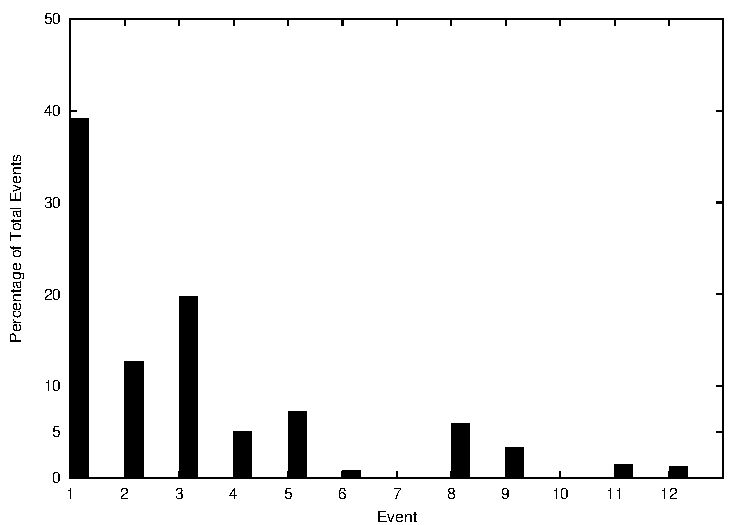
\includegraphics[width=3.5in]{all.pdf}
\end{center}
\caption{Percentage of total events that each individual event 
represents. For the type of event each number represents, see section~\ref{sec:historian}.}\label{fig:percents}
\end{figure}

The following results do not have any machine learning techniques 
being applied. These are baseline values obtained from a simulation
where the transitions happen completely randomly. The factory has been
initialized with one-hundred Senators, one Historian, and one President.
The complete simulation has been run one-hundred times, with the factory
being reset between each trial. 

~\fig{percents} shows each event and the percentage of total events that
this transition represents. To see what each number means, refer to 
section~\ref{sec:historian}. This table confirms many of our logical 
expectations about the system. Gathering support (event $1$) is the
most common state, as all other states have the option of going back to
this one. In theory, support gathering is supposed to be the most 
common activity that a Senator undergoes. Clearly, that is the case in 
practice as well. Because a Senator may only propose a bill to the floor
twice, the levels for presenting and voting on the floor are lower
than those activities in the committee phase. Since filibusters only
occur in extreme cases, they are only called for less than one percent
of the time. Likewise, the FBI will only catch a senator if they have committed a high number of scandals; therefore, this event occurs 
extremely rarely as well. 

\begin{figure}
\small
\begin{tabular}{l@{~}|r@{~}r@{~}@{~}r@{~}|c}
Event& 25\%& 50\% & 75\%&Quartiles\\\hline
Gather support& 389& 435& 974&  \boxplot{38.4}{39.8}{40.6}{43.2}{55.3}  \\
Present (Committee)& 118& 130& 294&  \boxplot{8.7}{11.8}{12.7}{13.4}{84.1}  \\
Vote (Committee)& 184& 200& 469&  \boxplot{13.0}{18.4}{19.7}{21.1}{75.8}  \\
Present (Floor)& 54& 59& 91&  \boxplot{1.3}{4.0}{5.1}{5.7}{92.9}  \\
Vote (Floor)& 70& 85& 164&  \boxplot{2.5}{6.0}{7.2}{8.2}{89.1}  \\
Scandal& 5& 9& 80&  \boxplot{0.1}{0.5}{0.8}{3.5}{94.6}  \\
Filibuster& 0& 1& 2& \boxplot{0.0}{0.0}{0.1}{0.2}{99.6}\\ 
Suspended& 0& 57& 100&  \boxplot{0.0}{0.0}{5.7}{9.8}{90.2} \\
Investigating& 29& 33& 79&  \boxplot{1.8}{2.8}{3.3}{3.7}{95.2}  \\
Caught by FBI& 0& 1& 8&  \boxplot{0.0}{0.0}{0.1}{0.3}{99.4} \\
Present (President)& 13& 19& 37&  \boxplot{0.5}{1.1}{1.5}{1.8}{96.6}  \\
Bill defeated& 9& 15& 54& \boxplot{0.0}{0.9}{1.3}{2.0}{96.4} \\\hline
\multicolumn{4}{c}{~}&~~~~~0~~~~~~~~50~~~~100
\end{tabular}
\caption{Events and the number of times they occur on an average 
simulation trial}\label{fig:quarts}
\end{figure}


~\fig{quarts} elaborates on this further. This table examines each 
action along with how often it occurs during the average run. The 
data points were collected from one-hundred trials and the 25, 
50, and 75 percentiles are reported. The quartile charts reflect those
numbers as percentages of total number of transitions.

Future oracles and learning tools should focus on when and how often
to trigger certain events. How often should a senator gather support?
When should they give a speech? When should a vote be called for? 
Scandals occur fairly rarely. It might be interesting to examine
when the benefit of committing a scandal outweighs the cost. It could
also be interesting to trigger a scenerio where the factory is not reset each "day." Instead, the senators that failed to pass their bills on the first
day could continue to hone them and gather support. Future progress will
examine some of these situations. 
 
\bibliographystyle{plain}
\bibliography{refs}
\end{document}
